\documentclass[11pt,oneside,noprintercorrection]{ustl}

%----------------------------------------------------------------------
%                     Chargement de quelques packages
%----------------------------------------------------------------------

% Si l'on veut produire une version PDF avec distiller ou pdflatex :
%\usepackage{tlhypref}
\usepackage[pdfborder=0 0 0]{ustl}
% Si l'on produit le PDF avec pdflatex, ceci remplace la plupart
% des polices EC par des polices CM, plus adaptees a la generation de PDF,
% car ayant des equivalents PS :
\usepackage{aeguill}


% Pour les figures PS :
\usepackage{graphicx}

% Si on veut des mini-tables des matieres (utiliser minitoc-hyper
% en conjonction avec tlhypref) :
\usepackage[french]{minitoc}
%\usepackage[french]{minitoc-hyper}

\usepackage[frenchb]{babel}
\usepackage{graphicx}
\usepackage{float}

% Pour les codes
\usepackage{listings}
\lstset{language=C++,basicstyle=\small}

\synctex = 1

%-------------------------------------------------------------------
%  Surcharge de commandes pour les variables et page d'en-t�te
%-------------------------------------------------------------------

\makeatletter

%
% les deux commandes suivantes sont entre \makeatletter
% et \makeatother parce qu'elles utilisent des `@'.
%

\renewcommand{\@DFD}{Universit� Lille 1}


\renewcommand{\@NancyIhe@d}{{\UseEntryFont{ThesisFirstPageHead}\noindent
    \centerline{\if@logo@uhp@
                    {\setbox0=\hbox{$\raise2.3cm\hbox{\UHPLogo}$}%
                     \ht0=\baselineskip\box0}\hfill
                \else
                    Universit� des Sciences et Technologies de Lille%
                \fi}%
    \@TL@cmn@head\\
    \par
    }%
    }


\newcommand\TheseLilleI{\renewcommand{\@ThesisFirstPageHead}{\@NancyIhe@d}%
                         \ThesisDiploma{{\UseEntryFont{ThesisDiploma}%
                              \\[3mm]
            {\UseEntryFont{ThesisSpecialty}( )}}}}

\makeatother

%-------------------------------------------------------------------
%           Corrections pour les imprimantes recto-verso
%                          (A AJUSTER)
%-------------------------------------------------------------------

%\ShiftOddPagesRight{-1mm}
%\ShiftOddPagesDown{2.5mm}
%\ShiftEvenPagesRight{0mm}
%\ShiftEvenPagesDown{0mm} 

%-------------------------------------------------------------------
%                Mise en page
%-------------------------------------------------------------------

%-------------------------------------------------------------------
%                             interligne
%-------------------------------------------------------------------
\renewcommand{\baselinestretch}{1.3}

%-------------------------------------------------------------------
%                             Marges
%-------------------------------------------------------------------

% pour positionner les vraies marges:
%\SetRealMargins{1mm}{1mm}

%-------------------------------------------------------------------
%                             En-tetes
%-------------------------------------------------------------------
%On n'utilise pas les logos
%\DontShowLogos

% Les en-tetes: quelques exemples
%\UppercaseHeadings
%\UnderlineHeadings
%\newcommand\bfheadings[1]{{\bf #1}}
%\FormatHeadingsWith{\bfheadings}
%\FormatHeadingsWith{\uppercase}
%\FormatHeadingsWith{\underline}
\newcommand\upun[1]{\uppercase{\underline{\underline{#1}}}}
\FormatHeadingsWith\upun

\newcommand\itheadings[1]{\textit{#1}}
\FormatHeadingsWith{\itheadings}

% pour avoir un trait sous l'en-tete:
\setlength{\HeadRuleWidth}{0.4pt}

%-------------------------------------------------------------------
%                Chemin d'inclusion des graphiques
%-------------------------------------------------------------------

\graphicspath{{img/}{./}}

%-------------------------------------------------------------------
%                         Les references
%-------------------------------------------------------------------

\NoChapterNumberInRef \NoChapterPrefix

%-------------------------------------------------------------------
%                           Brouillons
%-------------------------------------------------------------------

% ceci ajoute une marque `brouillon' et la date
%\ThesisDraft



\begin{document}
\renewcommand{\labelitemi}{$\bullet$}
\renewcommand{\labelitemii}{$\circ$}
%-------------------------------------------------------------------
%                          Encadrements
%-------------------------------------------------------------------

% encadre les chapitres dans la table des matieres:
% (ces commandes doivent figurer apres \begin{document}

%\FrameChaptersInToc
%\FramePartsInToc


%-------------------------------------------------------------------
%            Reinitialisation de la numerotation des chapitres
%-------------------------------------------------------------------

% Si la commande suivante est presente,
% elle doit figurer APRES \begin{document}
% et avant la premiere commande \part
\ResetChaptersAtParts

%-------------------------------------------------------------------
%               mini-tables des matieres par chapitre
%-------------------------------------------------------------------

% preparer les mini-tables des matieres par chapitre.
% (commande de minitoc.sty)
%\dominitoc

%-------------------------------------------------------------------
%                         Page de titre:
%-------------------------------------------------------------------


\ThesisKind{Rapport de projet XXX}
\ThesisPresentedThe{soutenu le XXXX}
\ThesisTitle{Titre du projet}
\ThesisAuthor{Nom du ou des auteurs}
%\NomDuLaboOuEntreprise{Nom labo ou entreprise}
%\LogoLaboOuEntreprise{alcove} % Image du logo du labo ou ets dans le rep img

\NomDuLaboOuEntreprise{}
\LogoLaboOuEntreprise{} % Image du logo du labo ou ets dans le rep img

\TheseLilleI

\NewJuryCategory{encadrant}{\it Encadrant :}
                        {\it Encadrants :}

%\encadrant = {Nom encadrant 1\\
%              Nom encadrant 2}

% Creation de la page de titre:
\MakeThesisTitlePage


%-------------------------------------------------------------------
%                  ecriture de `Chapitre' et `Partie'
%                      dans la table des matieres
%-------------------------------------------------------------------

\WritePartLabelInToc \WriteChapterLabelInToc

%-------------------------------------------------------------------
%                        table des matieres
%-------------------------------------------------------------------

\tableofcontents

%-------------------------------------------------------------------
%              Exemple d'utilisation de \SpecialSection
%-------------------------------------------------------------------

% La commande \mainmatter (nouvelle commande LaTeX2e) permet de passer
% a la numerotation arabe (ce que fait \pagenumbering{arabic})
% et de faire commencer la nouvelle page 1 sur une page impaire.
% On evitera donc d'utiliser directement \pagenumbering{arabic}.
\mainmatter

% ----------------------------------------------------------------
\SpecialSection{Introduction}



% Pour ne pas avoir le mot `Chapitre' au debut de chaque chapitre.
\NoChapterHead

XXXX


%--------------------------------------------------------------------------------------
%--------------------------------------------------------------------------------------
\chapter{Prise en main de \LaTeX}


\section{Similarit� par SSD}

1. La fonction iviComputeLeftSSDCost calcule la somme de distances carr�es  entre les deux images en prennant en compte un d�calage donn�. On va faire �a pour chaque valeur entre 0 et 32, et chaque fois on enregistre le resultat en mSSD. Apr�s chaque iteration, on compare les valeurs de mSSD et ceux de mMinSSD. Pour chaque valeur, dans mLeftDisparityMap on enregistrera le decalage qui correspond a mMinSSD

\section{V�rification gauche-droite}
2. Grace � ces instructions

pdPtr1 = mMinSSD.ptr<double>(iRow);
pdPtr2 = mSSD.ptr<double>(iRow);
pucDisparity = mLeftDisparityMap.ptr<unsigned char>(iRow);

On prends des pointeurs aux d�buts des images. En utilisant l'operateur increment, on change leur position selon leur type.

\section{Calcul efficace de SSD}
3. Dans le rapport, les autheurs prennent en compte la redondance pres�nte dans les calculs. Cette redondance est aussi pres�nte dans la m�thode vu en cours. Pour calculer le SSD d'un pixel, on fait des calculs d�j� fait en calculant le pixel pr�c�dent. Dans l'image \ref{fig:1} on voit que une grande partie des calculs effectu�s pour le pixel $(2,2)$ sont faites encore une fois pour la SSD du pixel $(2,3)$. 

\begin{figure}[!ht]
  \centering
  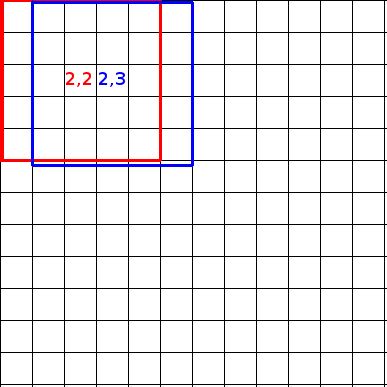
\includegraphics[height=4cm]{redundant.png}
  \caption{Calculs redundants}
  \label{fig:1}
\end{figure}

Pour eviter �a, les autheurs proposent de ne calculer que les nouvelles diffences carr�s. C'est evident qu'il ne faut que faire des calculs pour les pixels coch�s en vert dans la figure \ref{fig:2}

\begin{figure}[!ht]
  \centering
  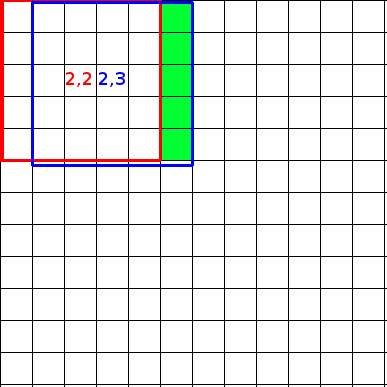
\includegraphics[height=4cm]{opt1.png}
  \caption{Calculs redundants}
  \label{fig:1}
\end{figure}

De plus, les autheurs utilisent aussI_{i la recursivit� pour eviter des r�p�titions en calculant les valeurs des colonnes.
On peut utiliser cette m�thode pour le calcul de la SSD en modifiant la fonction $P$.

$$
P(x,y,d)=(I_{l}(x,y)-I_{r}(x-d,y))^{2}
$$

Le nombre de calculs est determin� principalement par les appels recursifs � la fonction $Q(x,y,d)$. 
\SpecialSection{Conclusion}


\bibliographystyle{myunsrt}
\small
\bibliography{biblio}

\Annex{Annexe 1}

\end{document}
